%%  ***************************************************************************
%% My paper
%%
%% Authors: Emmett Brown, Marty McFly, Biff Tannen
%%
%% NOTE: this file will not compile until you called the script
%% generate-preamble.php once. See the file Readme.md to understand what
%% to do.
%%
%% This paper is an instance of the PaperShell template. For more
%% information, please visit https://github.com/sylvainhalle/PaperShell
%%  ***************************************************************************
%% ---------------------------
%% Author preamble. Uncomment the one corresponding to the
%% stylesheet you want. **Don't forget to also uncomment the proper
%% line for the postamble at the end!!**
%% ---------------------------
%\input preamble-aaai.inc.tex
\input preamble-acm.inc.tex
%\input preamble-acm-journal.inc.tex
%\input preamble-elsarticle.inc.tex
%\input preamble-ieee.inc.tex
%\input preamble-ieee-journal.inc.tex
%\input preamble-lncs.inc.tex
%\input preamble-svjour.inc.tex

%% ---------------------------
%% If you wish to include additional packages, define new environments or
%% new commands, put them in the file includes.tex
%%
%% Write your abstract in the file abstract.tex.
%% ---------------------------

%% ---------------------------
%% Categories and keywords. Uncomment only for ACM.
%% See: http://www.acm.org/about/class/ccs98-html
%% ---------------------------
\begin{comment}
  \category{D.2.2}{Software Engineering}{Design Tools and Techniques}
  \category{D.2.4}{Software Engineering}{Software/Program Verification}
  \category{H.3.5}{In\-for\-ma\-tion Storage and Retrieval}{Online Information Services}[web-based services]
  \terms{Theory, verification}
  \keywords{Navigation, web applications, model checking}
  \vfill\eject
\end{comment}

%% ---------------------------
%% Introduction
%% ---------------------------
\section{Introduction} %% {{{

M\ae{}cenas sodales ex in risus convallis elementum. Pr\ae{}sent at sem fermentum, egestas dolor non, ultrices elit. Cras at justo sit amet dolor lobortis blandit. Phasellus sodales erat eget tellus facilisis tristique. Nulla purus velit, hendrerit in cursus ut, euismod vit\ae{} odio. Morbi nec metus quis augue interdum ullamcorper ac at nisi. Nullam vit\ae{} imperdiet mauris. Nullam a ligula felis. Etiam at erat blandit nibh interdum posuere id at mi. Ut vit\ae{} ornare leo. Morbi vestibulum mauris id tellus volutpat, eget feugiat lorem maximus.

Donec maximus dui quis velit placerat auctor. Fusce vel tincidunt mi, vel porta eros. Fusce egestas purus sit amet ex hendrerit, at commodo justo rutrum. Nam interdum pharetra commodo. Duis ligula turpis, ultrices at posuere ac, posuere pretium eros. Ut vehicula sagittis quam eu luctus. Morbi lectus tortor, fermentum eu ultricies non, scelerisque et tortor. Mauris blandit gravida metus, sit amet consequat tortor finibus vel. Vivamus in sollicitudin nibh, eget maximus lorem. Mauris arcu leo, aliquet nec fringilla sed, auctor sit amet nunc. Lorem ipsum dolor sit amet, consectetur adipiscing elit. 

%% }}} --- Section

%% ---------------------------
%% A section
%% ---------------------------
\section{Donec id eros non nisl pharetra} %% {{{

In hendrerit commodo urna sit amet egestas. Phasellus ut faucibus diam. Etiam quis hendrerit augue. Nam vel arcu at massa iaculis ullamcorper. Sed in malesuada enim, ac rutrum augue \cite{Lenat83a}. Donec efficitur egestas massa in varius. Etiam at nibh commodo, iaculis massa nec, rutrum sem. Mauris imperdiet massa eu nibh fermentum, ac ultricies metus sollicitudin. Donec vel dolor non turpis efficitur rhoncus. M\ae{}cenas et augue congue elit viverra sagittis quis in magna. Vestibulum tempus tellus in efficitur viverra. Morbi vestibulum posuere tortor, vit\ae{} eleifend dolor iaculis id. Vestibulum ornare gravida tortor vel fermentum. Cras vulputate facilisis dui, non porttitor arcu blandit vel.

\begin{figure}
  \centering
  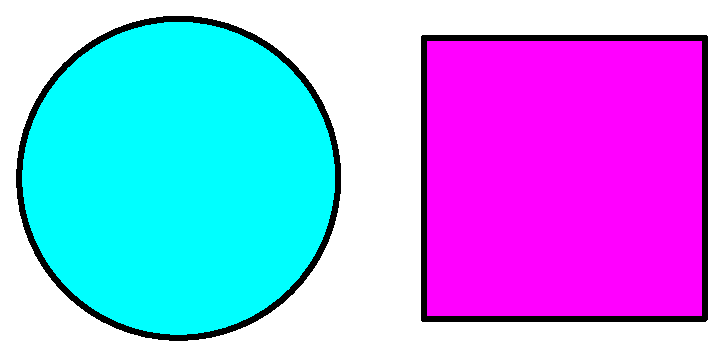
\includegraphics[width=0.4\textwidth]{square-circle}
  \caption{A square and a circle}
  \label{fig:square-circle}
\end{figure}

In maximus ante at metus vulputate congue. Sed eleifend ultrices tincidunt. Lorem ipsum dolor sit amet, consectetur adipiscing elit. Pr\ae{}sent quis rutrum elit. Nunc auctor nibh non sem consequat gravida. Nulla non dapibus metus. Cras viverra tempor nibh sit amet malesuada. Etiam non ante purus. M\ae{}cenas eleifend ultricies orci, ut fermentum erat suscipit elementum. Sed est libero, laoreet vel sodales ac, consectetur sed enim. Quisque hendrerit ac erat vit\ae{} posuere. Sed eros sapien, luctus ut justo lacinia, vestibulum sagittis lorem. Mauris porta dapibus dui, eu iaculis dolor faucibus id. 

%% }}} --- Section

%% ---------------------------
%% Bibliography. Uncomment the one corresponding to the
%% stylesheet you want.
%% ---------------------------
%\input postamble-aaai.inc.tex
\input postamble-acm.inc.tex
%\input postamble-acm-journal.inc.tex
%\input postamble-elsarticle.inc.tex
%\input postamble-ieee.inc.tex
%\input postamble-ieee-journal.inc.tex
%\input postamble-lncs.inc.tex
%\input postamble-svjour.inc.tex

\end{document}

%% :folding=explicit:wrap=soft:mode=latex:

